%%%%%%%%%%%%%%%%%%%%%%%%%%%%%%%%%%%%%%%%%%%%%%%%%%%%%%%%%%%%%%%%%%%%%%%
%% AGI-22 paper about temporal and procedural reasoning with OpenCog %%
%%%%%%%%%%%%%%%%%%%%%%%%%%%%%%%%%%%%%%%%%%%%%%%%%%%%%%%%%%%%%%%%%%%%%%%

\documentclass[runningheads]{llncs}
%
\usepackage{graphicx}
\usepackage{amsmath}
\usepackage{amssymb}
\usepackage{bussproofs}
\usepackage{cite}

% For ⩘ and ⩗ (requires the LuaLaTeX engine)
\usepackage{unicode-math}
\setmathfont{Stix Two Math}

% Commands for Atomese code
\newcommand{\SP}{\;\;\;}
\newcommand{\TTrue}{\textit{True}}
\newcommand{\TFalse}{\textit{False}}
\newcommand{\TAtom}{\textit{Atom}}
\newcommand{\TTime}{\textit{Time}}
\newcommand{\TEval}{\textit{Evaluation}}
\newcommand{\TList}{\textit{List}}
\newcommand{\TLamb}{\textit{Lambda}}
\newcommand{\TExec}{\textit{Execution}}
\newcommand{\TAtTime}{\textit{AtTime}}
\newcommand{\TAnd}{\textit{And}}
\newcommand{\TOr}{\textit{Or}}
\newcommand{\TNot}{\textit{Not}}
\newcommand{\TImpl}{\textit{Implication}}
\newcommand{\TPredImpl}{\textit{PredictiveImplication}}
\newcommand{\TSeqAnd}{\textit{SequentialAnd}}
\newcommand{\TSeqOr}{\textit{SequentialOr}}
\newcommand{\TBSeqAnd}{\textit{BackSequentialAnd}}
\newcommand{\TFSeqAnd}{\textit{ForeSequentialAnd}}
\newcommand{\TLag}{\textit{Lag}}
\newcommand{\TLead}{\textit{Lead}}
\newcommand{\TTV}{\textit{TV}}
\newcommand{\TTVPi}{\textit{TV}_i^P}
\newcommand{\TTVQi}{\textit{TV}_i^Q}
\newcommand{\TTVP}{\textit{TV}^P}
\newcommand{\TTVQ}{\textit{TV}^Q}
\newcommand{\TTVR}{\textit{TV}^R}
\newcommand{\TTVPQ}{\textit{TV}^{PQ}}
\newcommand{\TTVQR}{\textit{TV}^{QR}}
\newcommand{\TBTV}{\langle \TTV \rangle}
\newcommand{\TBTVPi}{\langle \TTVPi \rangle}
\newcommand{\TBTVQi}{\langle \TTVQi \rangle}
\newcommand{\TBTVP}{\langle \TTVP \rangle}
\newcommand{\TBTVQ}{\langle \TTVQ \rangle}
\newcommand{\TBTVR}{\langle \TTVR \rangle}
\newcommand{\TBTVPQ}{\langle \TTVPQ \rangle}
\newcommand{\TBTVQR}{\langle \TTVQR \rangle}
\newcommand{\Tstrength}{\textit s}
\newcommand{\Tconf}{\textit c}

% Commands for symbolic mathematical notations
\newcommand{\prob}{\mathbf{Pr}}
\newcommand{\limp}{\rightarrow}
\newcommand{\lpreimp}[1]{\leadsto^{#1}}
\newcommand{\lseqor}[1]{\bigslopedvee^{#1}}
\newcommand{\lseqand}[1]{\bigslopedwedge^{#1}}
\newcommand{\ldo}[1]{\widehat{#1}}
\newcommand{\llag}[2]{\overrightarrow{#1}^{#2}}
\newcommand{\llead}[2]{\overleftarrow{#1}^{#2}}
%% TODO: try to replace over right arrow by over right harp, etc
%% \newcommand{\llag}[2]{\accentset{\overrightharp}{#1}^{#2}}
%% \newcommand{\llead}[2]{\overleftharp{#1}^{#2}}

\begin{document}
%
\title{Rational OpenCog Controlled Agent}

%\titlerunning{Abbreviated paper title}
% If the paper title is too long for the running head, you can set
% an abbreviated paper title here
%
\author{Nil Geisweiller
  %\orcidID{0000-0001-5041-6299}
  \and Hedra Yusuf}
%
\authorrunning{N. Geisweiller et al.}
% First names are abbreviated in the running head.
% If there are more than two authors, 'et al.' is used.
%
\institute{ SingularityNET Foundation, The
  Netherlands\\ \email{\{nil,hedra\}@singularitynet.io}}
%
\maketitle              % typeset the header of the contribution
%

\begin{abstract}
  TODO

  \keywords{Symbolic Reinforcement Learning \and Procedural Reasoning
    \and OpenCog \and Minecraft}
\end{abstract}

\section{Introduction}

The goal of this project is to make an agent as rational as possible,
not necessarily as efficient as possible.  This stems from the concern
that in order to autonomously gain efficiency the agent must first be
able to make the best possible decisions, starting first in the outer
world, and then in the inner world.

% Inner actions could be as transitory as bringing a piece of
% knowledge to the attentional focus, and as profound as rewriting a
% part of its code, like a Goedel Machine.  The atomspace can be
% viewed as a very compact representation of an envelop over
% environments (cite partial operator induction paper).  And PLN can
% be viewed as an abstract-enabling way to calculate the cumulative
% reward (in case it is used as a re-inforcement learner) to be
% maximized, or a goal driven agent in a more general case.  For these
% reasons ROCCA may well be seen as an approximated combination of
% AI\Xi and a Goedel Machine.

The paper presents

The agent starts in a completely unknown environment

The idea is that reasoning is used at all levels, discovering patterns
from raw observations, building plans and making decisions.

It is a work in progress.

Neural networks are excellent at interpolation, but are rather poor at
extrapolation, what we need for true intelligence is a system that
thinks critically.

Rarely do causes and effects take place over arbitrary temporal
scales.  For instance it is unlikely to find a cause that may produce
the same effect, or an effect at all, after 1ms, 1 century or any time
in between.  For that reason we focus on a real time temporal logic.

\subsection{Related Work}

\subsection{Contributions}

The contributions of that paper are:
\begin{enumerate}
\item Design an architecture for controlling an agent based on that
  temporal reasoning extension.
\end{enumerate}

\subsection{Outline}

\begin{enumerate}
\item ROCCA
\item Minecraft experiment
\end{enumerate}

\section{Rational OpenCog Controlled Agent}

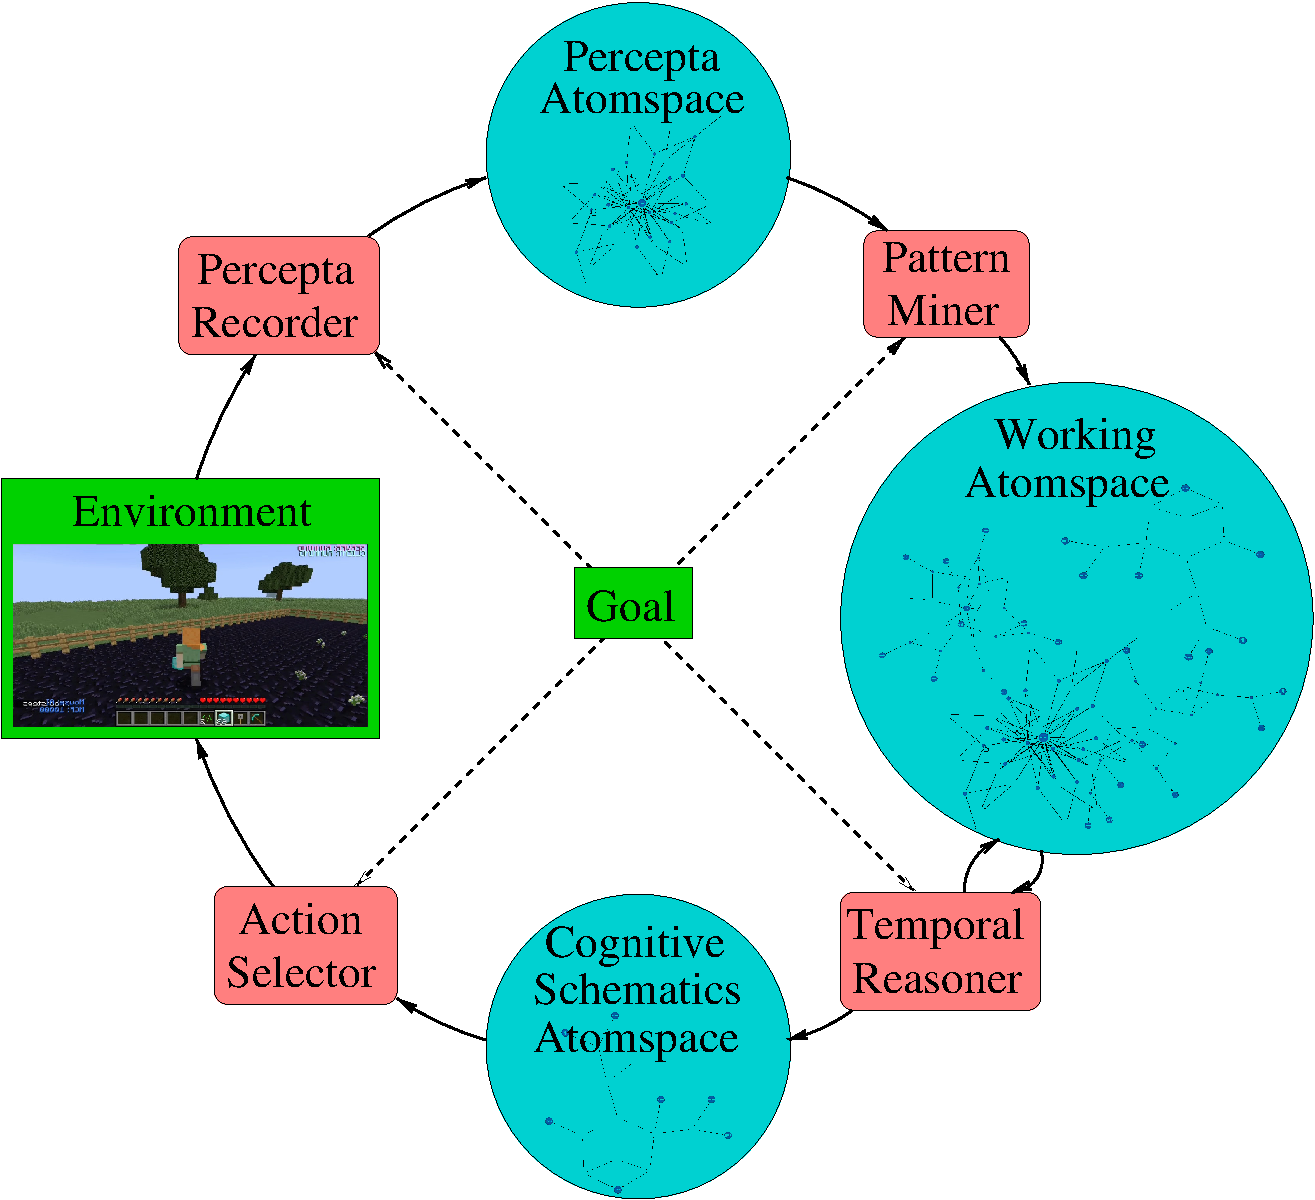
\includegraphics[width=1\textwidth]{pictures/rocca-chart-v0.6.pdf}

To experiment with temporal and procedural reasoning in the context of
embodied virtual agents in unknown environments we have implemented a
project called ROCCA, which stands for \emph{Rational OpenCog
Controlled Agent}.  ROCCA essentially acts as an interface between
virtual environments such as Malmo \cite{TODO} or OpenAI Gym
\cite{TODO} and OpenCog.  It provides an Observation-Planning-Action
control loop as well as various launchers to run OpenCog processes
such as PLN reasoning, pattern mining, etc.
%% During the life of the
%% agent control and learning phases are alternated to simulate a form of
%% online learning.
Provided a top goal, such as maximizing a reward, ROCCA orchestrates
the necessary learning and the planning to fulfill that goal.
%% somewhat like a reinforcement learning agent.
One may possibly see ROCCA as a reinforcement learning agent with the
particularity that learning and planning are, at least in principle,
entire done via reasoning.  In that respect it is similar in spirit to
OpenNARS for Applications (ONA) \cite{TODO} but uses PLN as its core
reasoning logic rather than NAL \cite{TODO}.
%% Where it differs from a typical
%% reinforcement learning agent in that both learning and planning are,

ROCCA is composed of two main processes, one for real-time agent
control and another one for non-reactive background learning.  In
principle these two processes could happen in parallel, though as of
right now they occur as distinct alternating phases.

\subsection{Control Phase}
The control phase is composed of control cycles, each decomposed into
Observation, Planning and Acting steps, more precisely
\begin{enumerate}
\item Observation step:
  \begin{enumerate}
  \item receives and timestamps observations from the environment,
  \item stores the timestamped observations in the atomspace.
  \end{enumerate}
\item Planning step:
  \begin{enumerate}
  \item selects the goal for that iteration,
  \item finds plans fulfilling that goal,
  \item given these plans, deduces a probabilistic distribution of
    actions,
  \item selects the next action according to the deduced probabilistic
    distribution.
  \end{enumerate}
\item Acting step:
  \begin{enumerate}
  \item timestamps and stores in the atomspace the selected action,
  \item runs the selected action and by that updates the environment,
  \item receives the reward from the environment,
  \item timestamps and stores the reward in the atomspace.
  \end{enumerate}
\end{enumerate}

None of these steps are difficult to carry with the exception of
deducing a probabilistic distribution of actions.  For that we use a
variation of Solomonoff induction described in \cite{TODO} which is
especially suited for plans described by conditional second order
distributions, in other words $\TPredImpl$ links.  More specifically
plans are $\TPredImpl$ links of the form
$$C \land A \lpreimp{T} G$$
called \emph{Cognitive Schematics}.  Which can be read as \emph{``in some
context $C$, if some action (elementary or composite) $A$ is executed,
then after $T$ time units, the goal $G$ is likely to be fulfilled''}.
The degree of expected fulfillment is specified by the truth value of
the $\TPredImpl$ link, not indicated in that notational format but
present in the extended Atomese format.  The difficulty then comes
down to discovering cognitive schematics that are as informative and
applicable as possible.

\subsection{Learning Phase}
As hinted above, the ultimate goal of the learning phase is to
discover maximally useful cognitive schematics, and by useful it is
specifically meant that they are as predictive and cover as many cases
as possible.

TODO: pattern mining and reasoning.

\section{Experiment with Simple Minecraft Environment}

In this experiment we built a minecraft environment using Malmo, which is a platform for Artificial Intelligence experimentation and research built on top of Minecraft. The demo environment consists of a small house with a locked door, diamonds inside and a key to get into the house. The agent, initially located outside of the house, can perform different actions like getting a key, opening a door of the house and collecting the diamonds in order to achieve a reward. \par
The aim of this experiment is to make the ROCCA agent learn from the actions and perceptions in the minecraft environment and do efficient planning so as to be able to collect as many diamonds as possible and accumulate reward. The ROCCA agent will be able to perform a series of possible actions with a goal of achieving a reward and learns from them by applying PLN (Probabilistic Logic Networks) and Pattern Miner, which can be seen as a specialized form of PLN reasoning. The Planning, the discovery of cognitive schematics, is also handled by PLN and its temporal reasoning rule base.

\begin{figure}[htbp]
\centerline{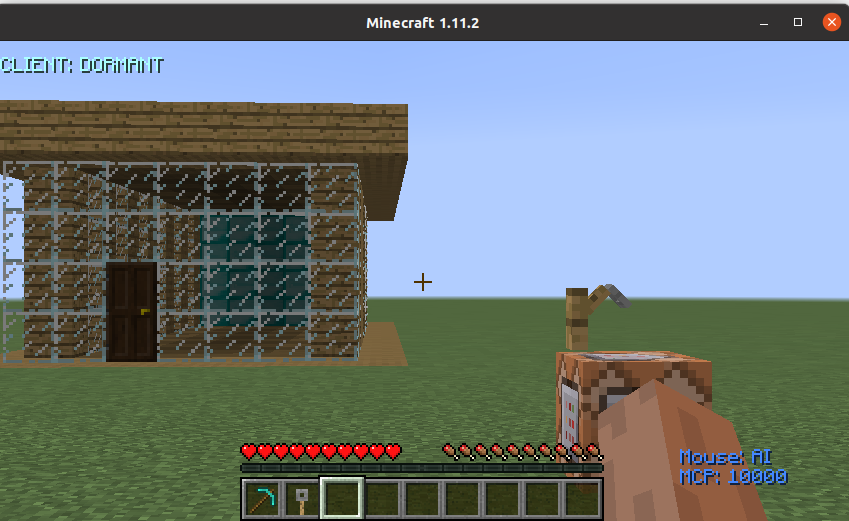
\includegraphics[scale=.2]{pictures/simple_demo.png}}
\caption{Simple Minecraft demo with a house and a key.}
\label{fig}
\end{figure}

There are lists of allowed actions provided by minecraft that an agent can perform like moving, turning, picking etc.. but due to the limited processing capacity we have to handle the observations from each action and to reduce complexity, we proposed to have an abstract action and perception where unnecessary details have been omitted. With that we generate three abstract actions namely go-to-key, go-to-house, go-to-diamonds where each of them contains a series of actions and returns an abstract perception about where the agent is (inside house, outside house, next to closed door etc..), about its inventory (has key, diamond pickaxe etc..) and the reward of completing a given action. \par
We perform various experiments tuning different parameters. A typical experiment has two iterations of the learning-training process with a duration of fifty iterations for each training. In the first cycle the agent will not have prior knowledge hence no learning will take place. The agent pursues the environment and builds its knowledge base by trying a combination of fifty randomly weighted actions. At the end of the first cycle the agent will have enough background knowledge to apply Pattern miner and PLN temporal reasoning. Hence, during the second cycle, the agent will be able to learn and plan the desired cognitive schematics which leads to a positive goal of getting a reward.\\
The ROCCA agent is able to learn the following cognitive schematics with higher strength.

$$\textit{outside}(\textit{self}, \textit{house}) \land \ldo{\textit{go\_to}(\textit{key})} \lpreimp{1} \textit{hold}(\textit{self}, \textit{key})$$
$$\textit{hold}(\textit{self}, \textit{key}) \land \ldo{\textit{go\_to}(\textit{house})} \lpreimp{1} \textit{inside}(\textit{self}, \textit{house})$$
$$\textit{inside}(\textit{self}, \textit{house}) \land \ldo{\textit{go\_to}(\textit{diamond})} \lpreimp{1} \textit{reward}(1)$$

In this experiment, we measure the agent's performance by the cognitive schematics learned and accumulated rewards achieved. The ROCAA agent is successful in learning the required cognitive schematics which leads the agent to collect more rewards in the second cycle. However, these findings with a simple minecraft environment with only few actions might not tell the overall performance of ROCCA. As a future work, further extensive experiments are needed to conclude the performance achieved.

\section{Conclusion}

%
% ---- Bibliography ----
%
\bibliographystyle{splncs04} \bibliography{local}

\end{document}
